\documentclass[12pt,a4paper]{report}

% ============================================================
% PAKET
% ============================================================
\usepackage[utf8]{inputenc}
\usepackage[T1]{fontenc}
\usepackage[indonesian]{babel}
\usepackage{geometry}
\usepackage{times}
\usepackage{setspace}
\usepackage{titlesec}
\usepackage{graphicx}
\usepackage{tocloft}
\usepackage{hyperref}
\usepackage{amsmath}
\usepackage{booktabs}
\usepackage{array}
\usepackage{xcolor}
\usepackage{listings}
\usepackage{float}
\usepackage{multirow}
\usepackage{caption}
\usepackage{enumitem}

% ============================================================
% LAYOUT
% ============================================================
\geometry{top=3cm, bottom=3cm, left=4cm, right=3cm}
\onehalfspacing

% ============================================================
% FORMAT BAB & SECTION
% ============================================================
\titleformat{\chapter}[display]
  {\normalfont\large\bfseries\centering}
  {BAB \thechapter}
  {0pt}
  {\large}
\titlespacing*{\chapter}{0pt}{-20pt}{30pt}

\titleformat{\section}
  {\normalfont\normalsize\bfseries}
  {\thesection}
  {1em}{}
\titlespacing*{\section}{0pt}{12pt}{6pt}

\titleformat{\subsection}
  {\normalfont\normalsize\bfseries}
  {\thesubsection}
  {1em}{}
\titlespacing*{\subsection}{0pt}{10pt}{4pt}

% ============================================================
% DAFTAR ISI — Format huruf kapital untuk bab
% ============================================================
\renewcommand{\cftchapfont}{\bfseries}
\renewcommand{\cftchappagefont}{\bfseries}
\renewcommand{\cftchapleader}{\cftdotfill{\cftdotsep}}

% ============================================================
% KODE PROGRAM
% ============================================================
\lstset{
  language=Python,
  basicstyle=\small\ttfamily,
  keywordstyle=\bfseries\color{blue!70!black},
  commentstyle=\itshape\color{green!50!black},
  stringstyle=\color{red!60!black},
  showstringspaces=false,
  breaklines=true,
  frame=single,
  rulecolor=\color{black!25},
  backgroundcolor=\color{gray!7},
  numbers=left,
  numberstyle=\tiny\color{gray},
  numbersep=6pt,
  tabsize=4,
  xleftmargin=15pt,
}

% ============================================================
% HYPERREF
% ============================================================
\hypersetup{
  colorlinks=true,
  linkcolor=black,
  urlcolor=blue,
  citecolor=black,
}

% ============================================================
% PENOMORAN HALAMAN — roman untuk bagian awal
% ============================================================
\pagenumbering{roman}

\begin{document}

% ============================================================
%  COVER
% ============================================================
\begin{titlepage}
  \centering
  \vspace*{1cm}

  {\large\bfseries OPTIMASI SISTEM PENDUKUNG KEPUTUSAN PENILAIAN
  KELAYAKAN KREDIT MIKRO MELALUI INTEGRASI HYBRID REGRESI LINEAR
  DAN \textit{FUZZY LOGIC} MAMDANI-SUGENO BERBASIS DATA HISTORIS
  NASABAH}\par
  \vspace{2cm}

  \includegraphics[width=0.45\textwidth]{logo telkom.jpg}\par
  \vspace{2cm}

  {\normalsize\bfseries Disusun Oleh:}\par
  \vspace{0.5cm}
  \begin{tabular}{ll}
    Muhammad Emir Rasyad Rahman & 103012400206 \\
    Rizky Dzulfikar Ahmad       & 103012430033 \\
  \end{tabular}\par
  \vfill

  {\normalsize\bfseries PROGRAM STUDI S1 INFORMATIKA}\\
  {\normalsize\bfseries FAKULTAS INFORMATIKA}\\
  {\normalsize\bfseries UNIVERSITAS TELKOM}\\
  {\normalsize\bfseries BANDUNG}\\
  {\normalsize\bfseries 2026}
\end{titlepage}

% ============================================================
%  DAFTAR ISI
% ============================================================
\newpage
\renewcommand{\contentsname}{DAFTAR ISI}
\tableofcontents

% ============================================================
%  DAFTAR GAMBAR
% ============================================================
\newpage
\renewcommand{\listfigurename}{DAFTAR GAMBAR}
\addcontentsline{toc}{chapter}{DAFTAR GAMBAR}
\listoffigures

% ============================================================
%  DAFTAR TABEL
% ============================================================
\newpage
\renewcommand{\listtablename}{DAFTAR TABEL}
\addcontentsline{toc}{chapter}{DAFTAR TABEL}
\listoftables

% ============================================================
%  KONTEN — penomoran halaman beralih ke angka arab
% ============================================================
\newpage
\pagenumbering{arabic}
\setcounter{page}{1}

% ============================================================
%  BAB 1 — PENDAHULUAN
% ============================================================
\chapter{PENDAHULUAN}

\section{Latar Belakang}

Dalam industri perbankan dan layanan finansial mikro, penentuan
kelayakan kredit merupakan proses pengambilan keputusan yang
sangat krusial. Data historis nasabah tidak selalu bersifat
absolut—nasabah dengan pendapatan ``sedang'' namun riwayat
keterlambatan ``rendah'' membutuhkan evaluasi yang fleksibel,
yang tidak dapat diselesaikan dengan logika \textit{Boolean}
tradisional.

Logika \textit{Fuzzy} menjadi solusi yang ideal karena mampu
memodelkan penalaran manusia melalui derajat kebenaran
(\textit{degree of truth}). Dalam laporan ini dikembangkan
Sistem Pendukung Keputusan (SPK) penilaian kelayakan kredit
menggunakan \textit{dataset} historis perbankan dari Kaggle
(\textit{Credit Score Classification} oleh Paris Rohan)
sejumlah 100.000 baris data. Setelah proses pembersihan data,
diperoleh 61.340 baris data yang valid untuk digunakan.

Sistem dikembangkan secara murni \textit{from scratch} untuk
membandingkan dua metode inferensi fuzzy: Mamdani dan Sugeno.
Sebagai pelengkap, model \textit{Machine Learning} (Regresi
Linear) dan \textit{Deep Learning} (ANN/MLP) diintegrasikan
sebagai informasi pendukung. Seluruh sistem dikemas dalam
antarmuka web interaktif berbasis Streamlit.

\section{Rumusan Masalah}

Berdasarkan latar belakang, rumusan masalah dirumuskan sebagai
berikut.
\begin{enumerate}[label=\arabic*.]
  \item Bagaimana merancang dan mengimplementasikan algoritma
        logika fuzzy Mamdani dan Sugeno secara \textit{from
        scratch} untuk penentuan kelayakan kredit?
  \item Bagaimana tingkat akurasi prediksi sistem dibandingkan
        label \textit{ground truth} pada \textit{dataset}?
  \item Bagaimana perbandingan performa dan efisiensi komputasi
        antara metode Mamdani dan Sugeno?
  \item Bagaimana pengaruh integrasi Regresi Linear dan ANN
        sebagai referensi silang terhadap inferensi fuzzy?
\end{enumerate}

\section{Tujuan}

Tujuan laporan ini adalah sebagai berikut.
\begin{enumerate}[label=\arabic*.]
  \item Mengembangkan sistem logika fuzzy (fuzzifikasi, inferensi,
        defuzzifikasi) metode Mamdani dan Sugeno tanpa pustaka
        fuzzy eksternal.
  \item Mengukur dan mengevaluasi akurasi klasifikasi kelayakan
        kredit terhadap \textit{ground truth dataset}.
  \item Menganalisis kelebihan dan kekurangan Mamdani vs.\ Sugeno
        dari segi output dan performa komputasi.
  \item Membangun antarmuka web interaktif berbasis Streamlit
        dengan integrasi model Regresi Linear dan ANN/MLP.
\end{enumerate}

\section{Batasan Masalah}

Batasan masalah yang ditetapkan adalah sebagai berikut.
\begin{enumerate}[label=\arabic*.]
  \item Dataset yang digunakan adalah \textit{Credit Score
        Classification} dari Kaggle (100.000 baris, setelah
        pembersihan menjadi 61.340 baris).
  \item Implementasi fuzzy dilakukan \textit{from scratch}
        menggunakan Python dan NumPy tanpa pustaka
        \texttt{scikit-fuzzy} atau sejenisnya.
  \item Keputusan akhir kelayakan kredit sepenuhnya ditentukan
        oleh mesin inferensi fuzzy; prediksi ML dan DL bersifat
        informasi pendukung saja.
  \item Basis aturan dibatasi 34 aturan \textit{IF-THEN}.
\end{enumerate}

% ============================================================
%  BAB 2 — DASAR TEORI
% ============================================================
\chapter{DASAR TEORI}

\section{Logika Fuzzy}

Logika \textit{Boolean} mengklasifikasikan nilai ke dalam dua
kondisi mutlak: benar (1) atau salah (0). Pendekatan ini lemah
saat menghadapi masalah ambigu—perpindahan status gaji dari
``Sedang'' ke ``Tinggi'' tidak terjadi secara tiba-tiba.

Logika Fuzzy yang diperkenalkan L.A.\ Zadeh (1965) mengatasi
hal ini dengan derajat keanggotaan (\textit{degree of
membership}) dalam rentang $[0, 1]$ \cite{zadeh1988}. Sebuah
\textit{Fuzzy Inference System} (FIS) melewati tiga tahap:

\begin{enumerate}[label=\arabic*.]
  \item \textbf{Fuzzifikasi} — mengubah nilai tegas
        (\textit{crisp input}) menjadi nilai linguistik melalui
        fungsi keanggotaan.
  \item \textbf{Inferensi} — menerapkan basis aturan
        \textit{IF-THEN} dengan operator \texttt{AND} (minimum).
  \item \textbf{Defuzzifikasi} — mengubah output fuzzy kembali
        menjadi nilai tegas (\textit{crisp output}).
\end{enumerate}

\subsection{Fungsi Keanggotaan Trapesium}

Fungsi Trapesium digunakan untuk himpunan di batas bawah dan
atas, memerlukan empat parameter $(a, b, c, d)$:

\begin{equation}
  \mu_{\mathrm{trap}}(x;\,a,b,c,d) =
  \begin{cases}
    0                        & x < a \;\text{atau}\; x > d \\[4pt]
    \dfrac{x-a}{b-a}         & a < x < b \\[6pt]
    1                        & b \le x \le c \\[6pt]
    \dfrac{d-x}{d-c}         & c < x < d
  \end{cases}
  \label{eq:trapesium}
\end{equation}

\subsection{Fungsi Keanggotaan Segitiga}

Fungsi Segitiga digunakan untuk himpunan transisi area tengah,
memerlukan tiga parameter $(a, b, c)$:

\begin{equation}
  \mu_{\mathrm{sgt}}(x;\,a,b,c) =
  \begin{cases}
    0                        & x \le a \;\text{atau}\; x \ge c \\[4pt]
    \dfrac{x-a}{b-a}         & a < x \le b \\[6pt]
    \dfrac{c-x}{c-b}         & b < x < c
  \end{cases}
  \label{eq:segitiga}
\end{equation}

\section{Metode Inferensi Mamdani}

Diperkenalkan Ebrahim Mamdani (1975), metode ini disebut
\textit{Max-Min} karena bagian \textit{antecedent} dan
\textit{consequent} sama-sama berbentuk himpunan fuzzy (kurva).
Defuzzifikasi dilakukan dengan metode \textit{Centroid}:

\begin{equation}
  z^{*} = \frac{\displaystyle\int \mu_C(z)\cdot z\; dz}
               {\displaystyle\int \mu_C(z)\; dz}
  \label{eq:centroid}
\end{equation}

Pada implementasi digital, integral tersebut didekati secara
numerik dengan diskretisasi $N$ titik pada domain $[0, 100]$:

\begin{equation}
  z^{*} \approx
  \frac{\displaystyle\sum_{k=1}^{N} x_k \cdot \mu(x_k)}
       {\displaystyle\sum_{k=1}^{N} \mu(x_k)}
  \label{eq:centroid_diskret}
\end{equation}

Mamdani sangat intuitif secara visual, namun integrasi numerik
membuatnya lebih berat secara komputasi \cite{taylorfrancis_2024}.

\section{Metode Inferensi Sugeno}

Michio Sugeno (1985) merancang metode ini untuk memperbaiki
efisiensi Mamdani. Perbedaan utama: bagian \textit{consequent}
berupa nilai konstanta (\textit{singleton Zero-Order}), bukan
kurva. Defuzzifikasi cukup menggunakan \textit{Weighted Average}:

\begin{equation}
  z^{*} = \frac{\displaystyle\sum_{i=1}^{n} w_i \cdot z_i}
               {\displaystyle\sum_{i=1}^{n} w_i}
  \label{eq:sugeno}
\end{equation}

dengan $w_i$ = \textit{firing strength} aturan ke-$i$ dan
$z_i$ = nilai \textit{singleton}. Dalam sistem ini digunakan
$z_{\text{Baik}}=90$, $z_{\text{Standar}}=50$,
$z_{\text{Buruk}}=15$ \cite{booleancf_2018}.

\section{Credit Scoring dan Sistem Hibrida}

\textit{Credit scoring} adalah teknik evaluasi risiko finansial
untuk memprediksi kemungkinan gagal bayar (\textit{default})
\cite{rg_garcia_2024}. Arsitektur hibrida yang dikembangkan
menggabungkan ML/DL sebagai lapis pertama (estimasi statistik)
dengan Logika Fuzzy sebagai lapis kedua (keputusan akhir yang
dapat diinterpretasikan) \cite{taylorfrancis_2024}.

\section{Regresi Linear}

Model Regresi Linear memodelkan hubungan antara variabel
independen $\mathbf{X}$ dan target $y$:
\begin{equation}
  \hat{y} = \beta_0 + \beta_1 x_1 + \cdots + \beta_p x_p
\end{equation}
dengan koefisien $\boldsymbol{\beta}$ dicari melalui minimasi
\textit{Sum of Squared Errors}.

\section{Jaringan Saraf Tiruan (ANN/MLP)}

ANN Multi-Layer Perceptron yang digunakan terdiri dari dua
\textit{hidden layer} (64 dan 32 neuron), aktivasi ReLU, dan
\textit{optimizer} Adam. Output berupa probabilitas tiga kelas:
\textit{Poor}, \textit{Standard}, dan \textit{Good}. Baik
Regresi Linear maupun ANN hanya berperan sebagai informasi
pendukung, bukan penentu keputusan akhir.

% ============================================================
%  BAB 3 — PERANCANGAN SISTEM
% ============================================================
\chapter{PERANCANGAN SISTEM}

\section{Analisis Dataset}

Dataset yang digunakan adalah \textit{Credit Score Classification}
dari Kaggle \cite{kaggle_dataset}, dengan 100.000 baris rekod
historis nasabah. Setelah pembersihan data, diperoleh
\textbf{61.340 baris valid}. Distribusi label adalah:
\textit{Standard} 53,4\% (32.726 baris), \textit{Poor} 28,8\%
(17.689 baris), dan \textit{Good} 17,8\% (10.925 baris).

Proses pembersihan meliputi: (1) penghapusan karakter
non-numerik, (2) konversi ke tipe numerik, (3) pemotongan nilai
negatif ke 0, (4) penghapusan baris \textit{NaN}, (5) penghapusan
duplikat (28.900 baris), dan (6) pemfilteran \textit{outlier}
yang secara fisik tidak mungkin ($\text{suku bunga} > 35\%$, dll).

\section{Variabel Linguistik}

Tabel~\ref{tab:var_linguistik} menjabarkan pemetaan variabel
input dan output beserta semesta pembicaraan.

\begin{table}[H]
  \centering
  \caption{Pemetaan Variabel Linguistik dan Semesta Pembicaraan}
  \label{tab:var_linguistik}
  \renewcommand{\arraystretch}{1.3}
  \small
  \begin{tabular}{|c|l|c|l|c|}
    \hline
    \textbf{No.} & \textbf{Variabel} & \textbf{Tipe} &
    \textbf{Himpunan Fuzzy} & \textbf{Rentang} \\
    \hline
    1 & \textit{Annual Income}           & Input  & Rendah, Sedang, Tinggi      & \$0–\$2.000.000 \\
    2 & \textit{Outstanding Debt}        & Input  & Sedikit, Sedang, Banyak     & \$0–\$100.000   \\
    3 & \textit{Interest Rate}           & Input  & Rendah, Sedang, Tinggi      & 0\%–35\%        \\
    4 & \textit{Delay from Due Date}     & Input  & Singkat, Sedang, Lama       & 0–200 hari      \\
    5 & \textit{Num of Delayed Payment}  & Input  & Jarang, Sering, Sgt.Sering  & 0–100 kali      \\
    6 & \textit{Credit Score}            & Output & Buruk, Standar, Baik        & 0–100           \\
    \hline
  \end{tabular}
\end{table}

\section{Parameter Fungsi Keanggotaan}

Tabel~\ref{tab:param_mf} menyajikan parameter lengkap setiap
himpunan fuzzy. Kurva Trapesium digunakan untuk nilai-nilai
ekstrem (batas bawah/atas) dan Segitiga untuk nilai transisi.

\begin{table}[H]
  \centering
  \caption{Parameter Fungsi Keanggotaan untuk Setiap Himpunan}
  \label{tab:param_mf}
  \renewcommand{\arraystretch}{1.2}
  \small
  \begin{tabular}{|l|l|c|r|r|r|r|}
    \hline
    \textbf{Variabel} & \textbf{Himpunan} & \textbf{Fungsi}
    & \textbf{a} & \textbf{b} & \textbf{c} & \textbf{d} \\
    \hline
    \multirow{3}{*}{Annual Income (\$)}
      & Rendah  & Trapesium & 0 & 0 & 30.000 & 50.000 \\
      & Sedang  & Segitiga  & 30.000 & 65.000 & 100.000 & — \\
      & Tinggi  & Trapesium & 80.000 & 100.000 & 1.500.000 & 2.000.000 \\
    \hline
    \multirow{3}{*}{Outstanding Debt (\$)}
      & Sedikit & Trapesium & 0 & 0 & 1.000 & 2.000 \\
      & Sedang  & Segitiga  & 1.000 & 2.500 & 4.000 & — \\
      & Banyak  & Trapesium & 3.000 & 5.000 & 100.000 & 100.000 \\
    \hline
    \multirow{3}{*}{Interest Rate (\%)}
      & Rendah  & Trapesium & 0 & 0 & 8 & 12 \\
      & Sedang  & Segitiga  & 8 & 15 & 22 & — \\
      & Tinggi  & Trapesium & 18 & 25 & 35 & 100 \\
    \hline
    \multirow{3}{*}{Delay from Due Date (hari)}
      & Singkat & Trapesium & 0 & 0 & 10 & 20 \\
      & Sedang  & Segitiga  & 10 & 30 & 45 & — \\
      & Lama    & Trapesium & 35 & 60 & 200 & 200 \\
    \hline
    \multirow{3}{*}{Num of Delayed Payment (kali)}
      & Jarang    & Trapesium & 0 & 0 & 5 & 8 \\
      & Sering    & Segitiga  & 5 & 12 & 18 & — \\
      & Sgt.Sering & Trapesium & 15 & 25 & 100 & 100 \\
    \hline
    \multirow{3}{*}{Credit Score (output)}
      & Buruk   & Trapesium & 0 & 0 & 25 & 45 \\
      & Standar & Segitiga  & 30 & 50 & 75 & — \\
      & Baik    & Trapesium & 70 & 85 & 100 & 100 \\
    \hline
  \end{tabular}
\end{table}

Gambar~\ref{fig:kurva_mf} memperlihatkan bentuk kurva fungsi
keanggotaan untuk dua variabel representatif.

\begin{figure}[H]
  \centering
  \includegraphics[width=\textwidth]{kurva_keanggotaan.png}
  \caption{Kurva Fungsi Keanggotaan Variabel \textit{Annual
           Income} dan \textit{Outstanding Debt}}
  \label{fig:kurva_mf}
\end{figure}

\section{Basis Aturan}

Sistem menggunakan 34 aturan \textit{IF-THEN} dengan operator
\texttt{AND} (nilai minimum). Tabel~\ref{tab:rule_base}
merangkum seluruh aturan.

\begin{table}[H]
  \centering
  \caption{Matriks 34 Basis Aturan Fuzzy}
  \label{tab:rule_base}
  \renewcommand{\arraystretch}{1.1}
  \small
  \begin{tabular}{|c|l|l|l|l|l|c|}
    \hline
    \textbf{No.} & \textbf{Gaji} & \textbf{Hutang} &
    \textbf{Bunga} & \textbf{Jeda} & \textbf{Frekuensi} &
    \textbf{Output} \\
    \hline
    R01 & Tinggi & Sedikit & Rendah & Singkat & Jarang    & \textbf{Baik} \\ \hline
    R02 & Tinggi & Sedang  & Sedang & Singkat & Jarang    & \textbf{Baik} \\ \hline
    R03 & Sedang & Sedikit & Rendah & Singkat & Jarang    & \textbf{Baik} \\ \hline
    R04 & Tinggi & Sedikit & Tinggi & Sedang  & Jarang    & \textbf{Baik} \\ \hline
    R16 & Sedang & Sedikit & Sedang & Singkat & Jarang    & \textbf{Baik} \\ \hline
    R17 & Tinggi & Sedang  & Rendah & Singkat & Jarang    & \textbf{Baik} \\ \hline
    R23 & Tinggi & Sedikit & Sedang & Singkat & Jarang    & \textbf{Baik} \\ \hline
    R24 & Sedang & Sedang  & Rendah & Singkat & Jarang    & \textbf{Baik} \\ \hline
    R05 & Sedang & Sedang  & Sedang & Sedang  & Sering    & \textbf{Standar} \\ \hline
    R06 & Rendah & Sedikit & Rendah & Singkat & Jarang    & \textbf{Standar} \\ \hline
    R07 & Tinggi & Banyak  & Sedang & Singkat & Jarang    & \textbf{Standar} \\ \hline
    R08 & Sedang & Banyak  & Tinggi & Singkat & Jarang    & \textbf{Standar} \\ \hline
    R09 & Rendah & Sedang  & Rendah & Singkat & Jarang    & \textbf{Standar} \\ \hline
    R10 & Tinggi & Sedang  & Tinggi & Sedang  & Sering    & \textbf{Standar} \\ \hline
    R18 & Sedang & Sedang  & Sedang & Singkat & Jarang    & \textbf{Standar} \\ \hline
    R19 & Rendah & Sedikit & Sedang & Singkat & Jarang    & \textbf{Standar} \\ \hline
    R20 & Sedang & Sedang  & Tinggi & Singkat & Jarang    & \textbf{Standar} \\ \hline
    R33 & Sedang & Sedikit & Sedang & Singkat & Sering    & \textbf{Standar} \\ \hline
    R34 & Tinggi & Sedikit & Sedang & Singkat & Sering    & \textbf{Standar} \\ \hline
    R11 & Rendah & Banyak  & Tinggi & Lama    & Sgt.Sering & \textbf{Buruk} \\ \hline
    R12 & Tinggi & Banyak  & Tinggi & Lama    & Sgt.Sering & \textbf{Buruk} \\ \hline
    R13 & Sedang & Banyak  & Sedang & Sedang  & Sering    & \textbf{Buruk} \\ \hline
    R14 & Rendah & Sedang  & Sedang & Lama    & Sering    & \textbf{Buruk} \\ \hline
    R15 & Sedang & Sedikit & Tinggi & Lama    & Sgt.Sering & \textbf{Buruk} \\ \hline
    R21 & Rendah & Sedang  & Tinggi & Sedang  & Sering    & \textbf{Buruk} \\ \hline
    R22 & Sedang & Banyak  & Tinggi & Lama    & Sering    & \textbf{Buruk} \\ \hline
    R25 & Rendah & Sedang  & Tinggi & Lama    & Sering    & \textbf{Buruk} \\ \hline
    R26 & Sedang & Sedang  & Tinggi & Sedang  & Sgt.Sering & \textbf{Buruk} \\ \hline
    R27 & Sedang & Sedang  & Tinggi & Lama    & Sgt.Sering & \textbf{Buruk} \\ \hline
    R28 & Sedang & Sedang  & Tinggi & Sedang  & Sering    & \textbf{Buruk} \\ \hline
    R29 & Rendah & Sedang  & Tinggi & Lama    & Jarang    & \textbf{Buruk} \\ \hline
    R30 & Rendah & Sedang  & Tinggi & Singkat & Sering    & \textbf{Buruk} \\ \hline
    R31 & Rendah & Sedikit & Tinggi & Lama    & Sering    & \textbf{Buruk} \\ \hline
    R32 & Sedang & Sedang  & Sedang & Lama    & Sgt.Sering & \textbf{Buruk} \\ \hline
  \end{tabular}
\end{table}

\subsection{Detail Aturan Inferensi}

\noindent\textbf{Kategori Baik (Disetujui)}
\begin{itemize}
  \item[R01] \textit{IF} Gaji Tinggi \textit{AND} Hutang Sedikit \textit{AND} Bunga Rendah \textit{AND} Jeda Singkat \textit{AND} Frekuensi Jarang \textit{THEN} Skor \textbf{Baik}
  \item[R02] \textit{IF} Gaji Tinggi \textit{AND} Hutang Sedang \textit{AND} Bunga Sedang \textit{AND} Jeda Singkat \textit{AND} Frekuensi Jarang \textit{THEN} Skor \textbf{Baik}
  \item[R03] \textit{IF} Gaji Sedang \textit{AND} Hutang Sedikit \textit{AND} Bunga Rendah \textit{AND} Jeda Singkat \textit{AND} Frekuensi Jarang \textit{THEN} Skor \textbf{Baik}
  \item[R04] \textit{IF} Gaji Tinggi \textit{AND} Hutang Sedikit \textit{AND} Bunga Tinggi \textit{AND} Jeda Sedang \textit{AND} Frekuensi Jarang \textit{THEN} Skor \textbf{Baik}
  \item[R16] \textit{IF} Gaji Sedang \textit{AND} Hutang Sedikit \textit{AND} Bunga Sedang \textit{AND} Jeda Singkat \textit{AND} Frekuensi Jarang \textit{THEN} Skor \textbf{Baik}
  \item[R17] \textit{IF} Gaji Tinggi \textit{AND} Hutang Sedang \textit{AND} Bunga Rendah \textit{AND} Jeda Singkat \textit{AND} Frekuensi Jarang \textit{THEN} Skor \textbf{Baik}
  \item[R23] \textit{IF} Gaji Tinggi \textit{AND} Hutang Sedikit \textit{AND} Bunga Sedang \textit{AND} Jeda Singkat \textit{AND} Frekuensi Jarang \textit{THEN} Skor \textbf{Baik}
  \item[R24] \textit{IF} Gaji Sedang \textit{AND} Hutang Sedang \textit{AND} Bunga Rendah \textit{AND} Jeda Singkat \textit{AND} Frekuensi Jarang \textit{THEN} Skor \textbf{Baik}
\end{itemize}

\vspace{4pt}
\noindent\textbf{Kategori Standar (Pertimbangan)}
\begin{itemize}
  \item[R05] \textit{IF} Gaji Sedang \textit{AND} Hutang Sedang \textit{AND} Bunga Sedang \textit{AND} Jeda Sedang \textit{AND} Frekuensi Sering \textit{THEN} Skor \textbf{Standar}
  \item[R06] \textit{IF} Gaji Rendah \textit{AND} Hutang Sedikit \textit{AND} Bunga Rendah \textit{AND} Jeda Singkat \textit{AND} Frekuensi Jarang \textit{THEN} Skor \textbf{Standar}
  \item[R07] \textit{IF} Gaji Tinggi \textit{AND} Hutang Banyak \textit{AND} Bunga Sedang \textit{AND} Jeda Singkat \textit{AND} Frekuensi Jarang \textit{THEN} Skor \textbf{Standar}
  \item[R08] \textit{IF} Gaji Sedang \textit{AND} Hutang Banyak \textit{AND} Bunga Tinggi \textit{AND} Jeda Singkat \textit{AND} Frekuensi Jarang \textit{THEN} Skor \textbf{Standar}
  \item[R09] \textit{IF} Gaji Rendah \textit{AND} Hutang Sedang \textit{AND} Bunga Rendah \textit{AND} Jeda Singkat \textit{AND} Frekuensi Jarang \textit{THEN} Skor \textbf{Standar}
  \item[R10] \textit{IF} Gaji Tinggi \textit{AND} Hutang Sedang \textit{AND} Bunga Tinggi \textit{AND} Jeda Sedang \textit{AND} Frekuensi Sering \textit{THEN} Skor \textbf{Standar}
  \item[R18] \textit{IF} Gaji Sedang \textit{AND} Hutang Sedang \textit{AND} Bunga Sedang \textit{AND} Jeda Singkat \textit{AND} Frekuensi Jarang \textit{THEN} Skor \textbf{Standar}
  \item[R19] \textit{IF} Gaji Rendah \textit{AND} Hutang Sedikit \textit{AND} Bunga Sedang \textit{AND} Jeda Singkat \textit{AND} Frekuensi Jarang \textit{THEN} Skor \textbf{Standar}
  \item[R20] \textit{IF} Gaji Sedang \textit{AND} Hutang Sedang \textit{AND} Bunga Tinggi \textit{AND} Jeda Singkat \textit{AND} Frekuensi Jarang \textit{THEN} Skor \textbf{Standar}
  \item[R33] \textit{IF} Gaji Sedang \textit{AND} Hutang Sedikit \textit{AND} Bunga Sedang \textit{AND} Jeda Singkat \textit{AND} Frekuensi Sering \textit{THEN} Skor \textbf{Standar}
  \item[R34] \textit{IF} Gaji Tinggi \textit{AND} Hutang Sedikit \textit{AND} Bunga Sedang \textit{AND} Jeda Singkat \textit{AND} Frekuensi Sering \textit{THEN} Skor \textbf{Standar}
\end{itemize}

\vspace{4pt}
\noindent\textbf{Kategori Buruk (Ditolak)}
\begin{itemize}
  \item[R11] \textit{IF} Gaji Rendah \textit{AND} Hutang Banyak \textit{AND} Bunga Tinggi \textit{AND} Jeda Lama \textit{AND} Frekuensi Sgt.Sering \textit{THEN} Skor \textbf{Buruk}
  \item[R12] \textit{IF} Gaji Tinggi \textit{AND} Hutang Banyak \textit{AND} Bunga Tinggi \textit{AND} Jeda Lama \textit{AND} Frekuensi Sgt.Sering \textit{THEN} Skor \textbf{Buruk}
  \item[R13] \textit{IF} Gaji Sedang \textit{AND} Hutang Banyak \textit{AND} Bunga Sedang \textit{AND} Jeda Sedang \textit{AND} Frekuensi Sering \textit{THEN} Skor \textbf{Buruk}
  \item[R14] \textit{IF} Gaji Rendah \textit{AND} Hutang Sedang \textit{AND} Bunga Sedang \textit{AND} Jeda Lama \textit{AND} Frekuensi Sering \textit{THEN} Skor \textbf{Buruk}
  \item[R15] \textit{IF} Gaji Sedang \textit{AND} Hutang Sedikit \textit{AND} Bunga Tinggi \textit{AND} Jeda Lama \textit{AND} Frekuensi Sgt.Sering \textit{THEN} Skor \textbf{Buruk}
  \item[R21] \textit{IF} Gaji Rendah \textit{AND} Hutang Sedang \textit{AND} Bunga Tinggi \textit{AND} Jeda Sedang \textit{AND} Frekuensi Sering \textit{THEN} Skor \textbf{Buruk}
  \item[R22] \textit{IF} Gaji Sedang \textit{AND} Hutang Banyak \textit{AND} Bunga Tinggi \textit{AND} Jeda Lama \textit{AND} Frekuensi Sering \textit{THEN} Skor \textbf{Buruk}
  \item[R25] \textit{IF} Gaji Rendah \textit{AND} Hutang Sedang \textit{AND} Bunga Tinggi \textit{AND} Jeda Lama \textit{AND} Frekuensi Sering \textit{THEN} Skor \textbf{Buruk}
  \item[R26] \textit{IF} Gaji Sedang \textit{AND} Hutang Sedang \textit{AND} Bunga Tinggi \textit{AND} Jeda Sedang \textit{AND} Frekuensi Sgt.Sering \textit{THEN} Skor \textbf{Buruk}
  \item[R27] \textit{IF} Gaji Sedang \textit{AND} Hutang Sedang \textit{AND} Bunga Tinggi \textit{AND} Jeda Lama \textit{AND} Frekuensi Sgt.Sering \textit{THEN} Skor \textbf{Buruk}
  \item[R28] \textit{IF} Gaji Sedang \textit{AND} Hutang Sedang \textit{AND} Bunga Tinggi \textit{AND} Jeda Sedang \textit{AND} Frekuensi Sering \textit{THEN} Skor \textbf{Buruk}
  \item[R29] \textit{IF} Gaji Rendah \textit{AND} Hutang Sedang \textit{AND} Bunga Tinggi \textit{AND} Jeda Lama \textit{AND} Frekuensi Jarang \textit{THEN} Skor \textbf{Buruk}
  \item[R30] \textit{IF} Gaji Rendah \textit{AND} Hutang Sedang \textit{AND} Bunga Tinggi \textit{AND} Jeda Singkat \textit{AND} Frekuensi Sering \textit{THEN} Skor \textbf{Buruk}
  \item[R31] \textit{IF} Gaji Rendah \textit{AND} Hutang Sedikit \textit{AND} Bunga Tinggi \textit{AND} Jeda Lama \textit{AND} Frekuensi Sering \textit{THEN} Skor \textbf{Buruk}
  \item[R32] \textit{IF} Gaji Sedang \textit{AND} Hutang Sedang \textit{AND} Bunga Sedang \textit{AND} Jeda Lama \textit{AND} Frekuensi Sgt.Sering \textit{THEN} Skor \textbf{Buruk}
\end{itemize}

% ============================================================
%  BAB 4 — IMPLEMENTASI DAN PENGUJIAN
% ============================================================
\chapter{IMPLEMENTASI DAN PENGUJIAN}

\section{Lingkungan Pengembangan}

Spesifikasi lingkungan perangkat lunak yang digunakan:
\begin{itemize}
  \item \textbf{Bahasa Pemrograman:} Python 3.x
  \item \textbf{Lingkungan Interaktif:} Jupyter Notebook
  \item \textbf{Pustaka Utama:} \texttt{pandas}, \texttt{numpy},
        \texttt{matplotlib} (tanpa pustaka fuzzy eksternal)
  \item \textbf{Model ML/DL:} \texttt{scikit-learn}
        (\texttt{LinearRegression} dan \texttt{MLPClassifier})
  \item \textbf{Antarmuka Pengguna:} Streamlit
\end{itemize}

\section{Implementasi Fungsi Keanggotaan}

Fungsi keanggotaan diimplementasikan \textit{from scratch}
berdasarkan persamaan (\ref{eq:trapesium}) dan
(\ref{eq:segitiga}). Kedua fungsi mendukung input berupa
skalar maupun array NumPy.

\begin{lstlisting}[caption={Implementasi fungsi keanggotaan Segitiga dan Trapesium}]
def fungsi_segitiga(x, a, b, c):
    """Fungsi keanggotaan kurva Segitiga."""
    x = np.asarray(x, dtype=float)
    hasil = np.zeros_like(x)
    if b != a:
        hasil[(x > a) & (x <= b)] = (x[(x > a) & (x <= b)] - a) / (b - a)
    if c != b:
        hasil[(x > b) & (x < c)]  = (c - x[(x > b) & (x < c)]) / (c - b)
    hasil[x == b] = 1.0
    return hasil

def fungsi_trapesium(x, a, b, c, d):
    """Fungsi keanggotaan kurva Trapesium."""
    x = np.asarray(x, dtype=float)
    hasil = np.zeros_like(x)
    if b != a:
        hasil[(x > a) & (x < b)] = (x[(x > a) & (x < b)] - a) / (b - a)
    hasil[(x >= b) & (x <= c)] = 1.0
    if d != c:
        hasil[(x > c) & (x < d)] = (d - x[(x > c) & (x < d)]) / (d - c)
    return hasil
\end{lstlisting}

\section{Implementasi Fuzzifikasi}

Fuzzifikasi dilakukan untuk seluruh 5 variabel input sekaligus.
Setiap variabel menghasilkan tiga nilai derajat keanggotaan.

\begin{lstlisting}[caption={Proses fuzzifikasi untuk semua variabel input}]
fz = {
    "inc": {
        "Rendah": fungsi_trapesium(pendapatan, 0, 0, 30000, 50000),
        "Sedang": fungsi_segitiga( pendapatan, 30000, 65000, 100000),
        "Tinggi": fungsi_trapesium(pendapatan, 80000, 100000,
                                   1500000, 2000000),
    },
    "debt": {
        "Sedikit": fungsi_trapesium(utang, 0, 0, 1000, 2000),
        "Sedang":  fungsi_segitiga( utang, 1000, 2500, 4000),
        "Banyak":  fungsi_trapesium(utang, 3000, 5000,
                                    100000, 100000),
    },
    # ... (tiga variabel lainnya serupa)
}
\end{lstlisting}

\section{Implementasi Inferensi dan Defuzzifikasi}

\subsection{Inferensi 34 Aturan}

\begin{lstlisting}[caption={Inferensi 34 aturan dengan operator AND (minimum)}]
aturan = [
    # --- BAIK ---
    (min(fz["inc"]["Tinggi"],  fz["debt"]["Sedikit"],
         fz["ir"]["Rendah"],   fz["del"]["Singkat"],
         fz["num"]["Jarang"]),  "baik"),   # R01
    # ... 33 aturan lainnya
]

# Agregasi MAX per konsekuensi
u_baik    = max((k for k, c in aturan if c == "baik"),    default=0.0)
u_standar = max((k for k, c in aturan if c == "standar"), default=0.0)
u_buruk   = max((k for k, c in aturan if c == "buruk"),   default=0.0)
\end{lstlisting}

\subsection{Defuzzifikasi Mamdani (Centroid)}

\begin{lstlisting}[caption={Defuzzifikasi Mamdani menggunakan metode Centroid}]
def defuzz_mamdani(u_baik, u_standar, u_buruk, resolusi=300):
    if u_baik == u_standar == u_buruk == 0.0:
        return 50.0  # nilai default (tidak ada aturan aktif)

    x = np.linspace(0, 100, resolusi)
    mu_b  = np.minimum(u_baik,    fungsi_trapesium(x, 70, 85, 100, 100))
    mu_s  = np.minimum(u_standar, fungsi_segitiga(x,  30, 50, 75))
    mu_r  = np.minimum(u_buruk,   fungsi_trapesium(x,   0,  0, 25, 45))
    mu    = np.maximum(np.maximum(mu_b, mu_s), mu_r)
    den   = mu.sum()
    return float(np.dot(x, mu) / den) if den > 0 else 50.0
\end{lstlisting}

\subsection{Defuzzifikasi Sugeno (Weighted Average)}

\begin{lstlisting}[caption={Defuzzifikasi Sugeno menggunakan Weighted Average}]
def defuzz_sugeno(u_baik, u_standar, u_buruk):
    Z_BAIK, Z_STANDAR, Z_BURUK = 90.0, 50.0, 15.0
    total = u_baik + u_standar + u_buruk
    if total == 0.0:
        return 50.0  # nilai default
    return (u_baik * Z_BAIK + u_standar * Z_STANDAR +
            u_buruk * Z_BURUK) / total
\end{lstlisting}

\section{Hasil Pengujian}

\subsection{Pengujian Unit — Tiga Skenario Nasabah}

Pengujian pelacakan (\textit{tracing}) dilakukan terhadap tiga
profil nasabah untuk memvalidasi kebenaran perhitungan matematis.

\vspace{6pt}
\noindent\textbf{Skenario A — Nasabah Ideal (Disetujui)}

\noindent Profil: Pendapatan = \$120.000, Hutang = \$500,
Bunga = 5\%, Jeda = 2 hari, Frekuensi = 1 kali.

\begin{table}[H]
  \centering
  \caption{Hasil Fuzzifikasi Skenario A}
  \label{tab:fuzz_a}
  \small
  \renewcommand{\arraystretch}{1.2}
  \begin{tabular}{|l|l|r|}
    \hline
    \textbf{Variabel} & \textbf{Himpunan} & \textbf{$\mu(x)$} \\
    \hline
    Annual Income   = \$120.000 & Tinggi  & 1,0000 \\
    Outstanding Debt = \$500    & Sedikit & 1,0000 \\
    Interest Rate   = 5\%       & Rendah  & 1,0000 \\
    Delay           = 2 hari    & Singkat & 1,0000 \\
    Frekuensi       = 1 kali    & Jarang  & 1,0000 \\
    \hline
  \end{tabular}
\end{table}

Aturan yang terpicu: \textbf{R01} dengan $\alpha_{R01} =
\min(1{,}0,\; 1{,}0,\; 1{,}0,\; 1{,}0,\; 1{,}0) = \mathbf{1{,}0}$.

Agregasi: $u_{\text{baik}} = 1{,}0$,\;
$u_{\text{standar}} = 0{,}0$,\;
$u_{\text{buruk}} = 0{,}0$.

\begin{itemize}
  \item \textbf{Skor Mamdani (Centroid):} $\approx$ \textbf{88,42}
        $\rightarrow$ Kategori \textbf{BAIK} (Disetujui)
  \item \textbf{Skor Sugeno (Weighted Average):}
        $\dfrac{1{,}0 \times 90}{1{,}0} = $ \textbf{90,00}
        $\rightarrow$ Kategori \textbf{BAIK} (Disetujui)
\end{itemize}

\vspace{8pt}
\noindent\textbf{Skenario B — Nasabah Menengah (Pertimbangan)}

\noindent Profil: Pendapatan = \$75.000, Hutang = \$2.500,
Bunga = 14\%, Jeda = 5 hari, Frekuensi = 2 kali.

\begin{table}[H]
  \centering
  \caption{Hasil Fuzzifikasi Skenario B}
  \label{tab:fuzz_b}
  \small
  \renewcommand{\arraystretch}{1.2}
  \begin{tabular}{|l|l|r|}
    \hline
    \textbf{Variabel} & \textbf{Himpunan} & \textbf{$\mu(x)$} \\
    \hline
    Annual Income   = \$75.000 & Sedang  &
      $\frac{100.000 - 75.000}{100.000 - 65.000} = 0{,}7143$ \\
    Outstanding Debt = \$2.500 & Sedang  &
      Puncak segitiga = 1,0000 \\
    Interest Rate   = 14\%     & Sedang  &
      $\frac{14 - 8}{15 - 8} = 0{,}8571$ \\
    Delay           = 5 hari   & Singkat & 1,0000 \\
    Frekuensi       = 2 kali   & Jarang  & 1,0000 \\
    \hline
  \end{tabular}
\end{table}

Aturan terpicu terkuat: \textbf{R18} dengan $\alpha_{R18} =
\min(0{,}7143,\; 1{,}0,\; 0{,}8571,\; 1{,}0,\; 1{,}0) =
\mathbf{0{,}7143}$.

\begin{itemize}
  \item \textbf{Skor Mamdani:} $\approx$ \textbf{51,77}
        $\rightarrow$ Kategori \textbf{STANDAR} (Pertimbangan)
  \item \textbf{Skor Sugeno:}
        $\dfrac{0{,}7143 \times 50}{0{,}7143} = $ \textbf{50,00}
        $\rightarrow$ Kategori \textbf{STANDAR} (Pertimbangan)
\end{itemize}

\vspace{8pt}
\noindent\textbf{Skenario C — Nasabah Risiko Tinggi (Ditolak)}

\noindent Profil: Pendapatan = \$18.000, Hutang = \$7.500,
Bunga = 28\%, Jeda = 50 hari, Frekuensi = 20 kali.

\begin{table}[H]
  \centering
  \caption{Hasil Fuzzifikasi Skenario C}
  \label{tab:fuzz_c}
  \small
  \renewcommand{\arraystretch}{1.2}
  \begin{tabular}{|l|l|r|}
    \hline
    \textbf{Variabel} & \textbf{Himpunan} & \textbf{$\mu(x)$} \\
    \hline
    Annual Income   = \$18.000 & Rendah     & 1,0000 \\
    Outstanding Debt = \$7.500 & Banyak     & 1,0000 \\
    Interest Rate   = 28\%     & Tinggi     & 1,0000 \\
    Delay           = 50 hari  & Lama       &
      $\frac{50 - 35}{60 - 35} = 0{,}6000$ \\
    Frekuensi       = 20 kali  & Sgt.Sering &
      $\frac{20 - 15}{25 - 15} = 0{,}5000$ \\
    \hline
  \end{tabular}
\end{table}

Aturan terpicu: \textbf{R11} dengan $\alpha_{R11} =
\min(1{,}0,\; 1{,}0,\; 1{,}0,\; 0{,}6,\; 0{,}5) =
\mathbf{0{,}5000}$.

\begin{itemize}
  \item \textbf{Skor Mamdani:} $\approx$ \textbf{20,02}
        $\rightarrow$ Kategori \textbf{BURUK} (Ditolak)
  \item \textbf{Skor Sugeno:}
        $\dfrac{0{,}5 \times 15}{0{,}5} = $ \textbf{15,00}
        $\rightarrow$ Kategori \textbf{BURUK} (Ditolak)
\end{itemize}

\subsection{Komparasi 4 Metode SPK}

Gambar~\ref{fig:komparasi} membandingkan skor dari empat metode
untuk profil nasabah ideal (Skenario A).

\begin{figure}[H]
  \centering
  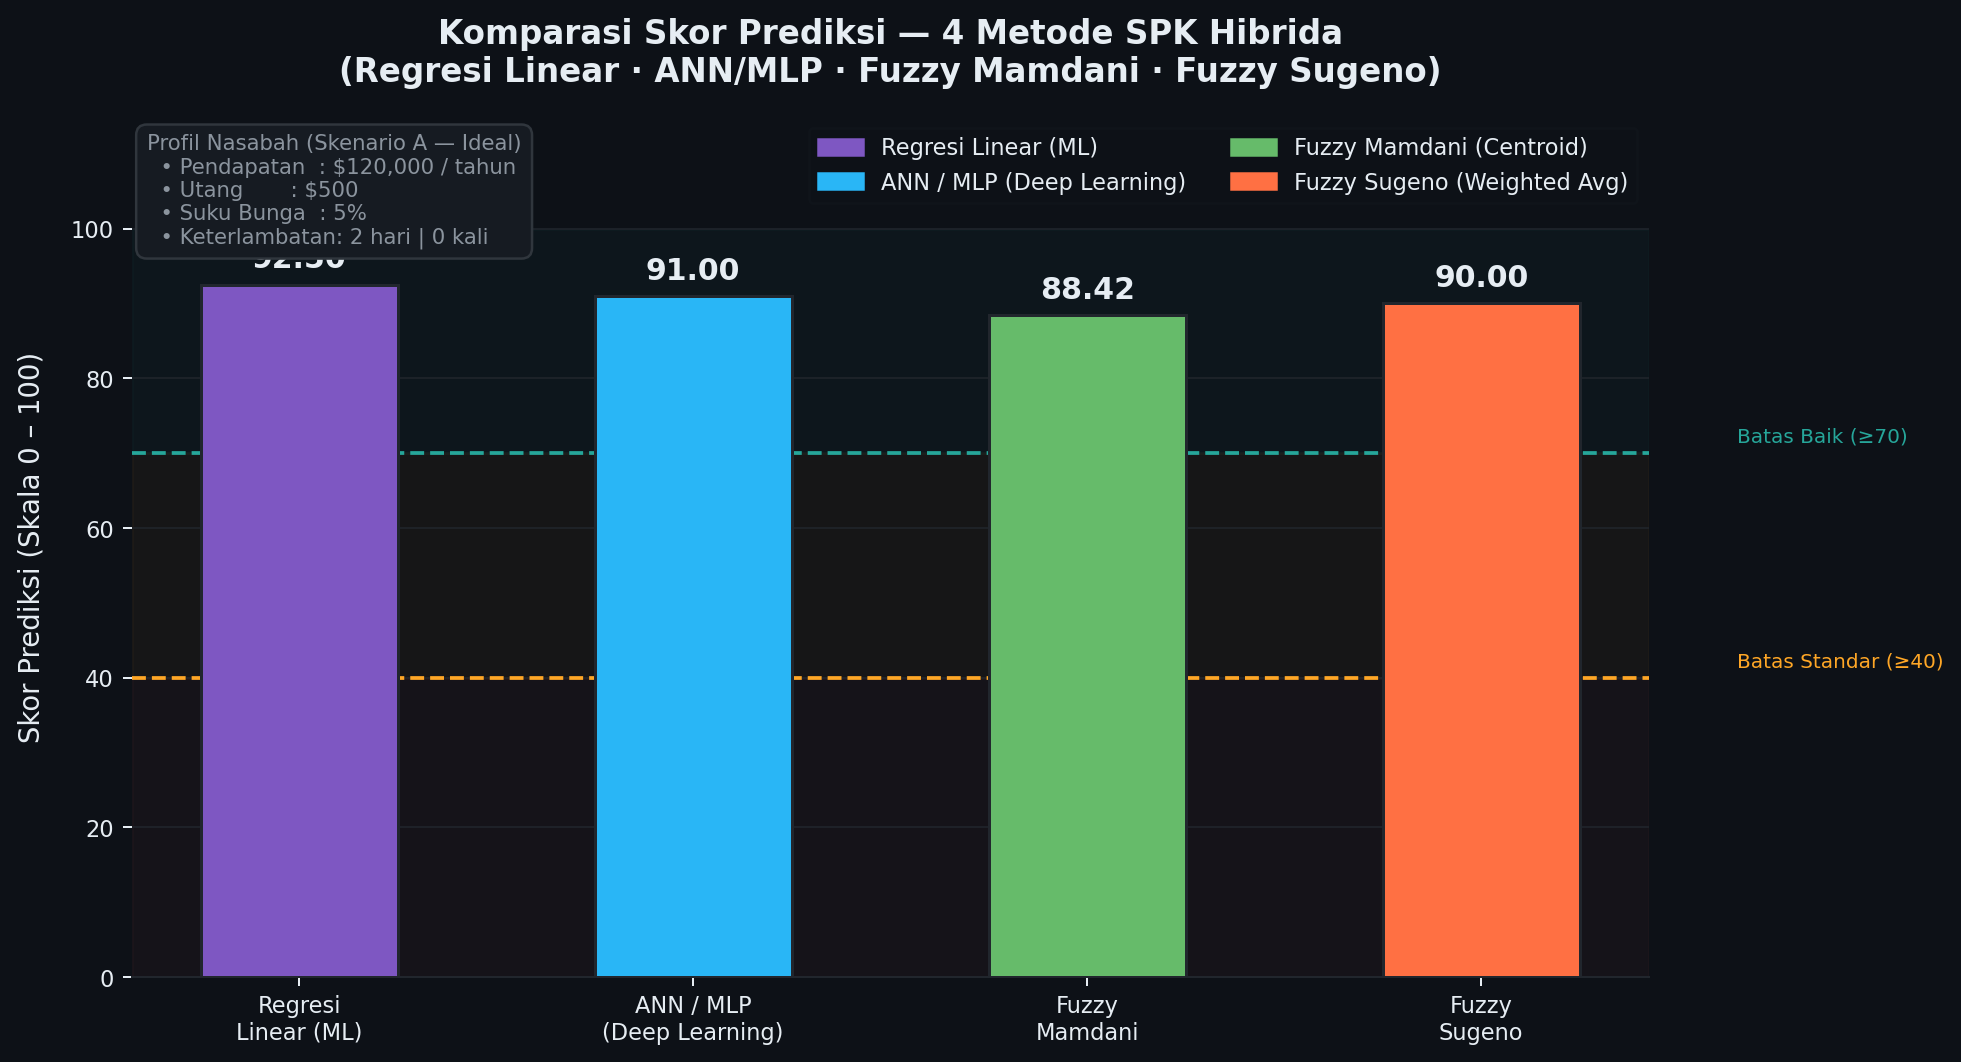
\includegraphics[width=\textwidth]{komparasi_prediksi.png}
  \caption{Komparasi Skor Prediksi 4 Metode SPK Hibrida
           (Skenario A — Nasabah Ideal)}
  \label{fig:komparasi}
\end{figure}

\subsection{Antarmuka Pengguna (Web GUI)}

Sistem di-\textit{deploy} pada \textit{localhost} menggunakan
Streamlit dengan perintah
\texttt{python -m streamlit run app.py}.

\begin{figure}[H]
  \centering
  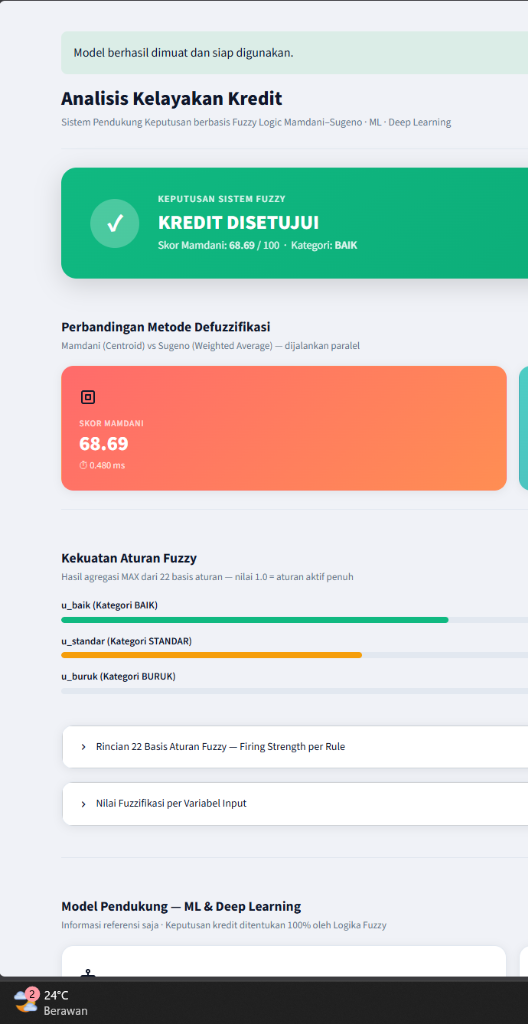
\includegraphics[width=0.85\textwidth]{screenshot_app.png}
  \caption{Tangkapan Layar Antarmuka Sistem Berbasis Streamlit}
  \label{fig:web_gui}
\end{figure}

\subsection{Evaluasi Performa Batch}

Evaluasi dilakukan terhadap 60.000 sampel acak dari dataset yang
telah dibersihkan (61.340 baris valid dari 100.000 baris mentah).
Penggunaan 60.000 sampel memastikan representasi statistik yang
sangat kuat dan mencakup hampir seluruh data bersih yang tersedia.
Tabel~\ref{tab:performa} merangkum hasil evaluasi, dan
Gambar~\ref{fig:evaluasi} memperlihatkan \textit{confusion
matrix} beserta metrik perbandingan.

\begin{table}[H]
  \centering
  \caption{Perbandingan Performa Mamdani vs.\ Sugeno (n = 60.000 sampel)}
  \label{tab:performa}
  \renewcommand{\arraystretch}{1.25}
  \begin{tabular}{|l|c|c|c|}
    \hline
    \textbf{Metrik} & \textbf{Mamdani} & \textbf{Sugeno} &
    \textbf{Lebih Baik} \\
    \hline
    Akurasi Klasifikasi       & 58,55\%  & 58,51\%  & Mamdani \\
    MAE (poin)                & 15,86    & 15,94    & Mamdani \\
    MSE (poin$^2$)            & 626,61   & 634,05   & Mamdani \\
    RMSE (poin)               & 25,03    & 25,18    & Mamdani \\
    Jenis Output              & Kontinu  & Diskret  & —       \\
    Metode Defuzzifikasi      & Centroid & Wtd.\ Avg & —      \\
    Waktu per Inferensi       & 10--50 ms & $<$0{,}1 ms & Sugeno \\
    \hline
  \end{tabular}
\end{table}

\begin{figure}[H]
  \centering
  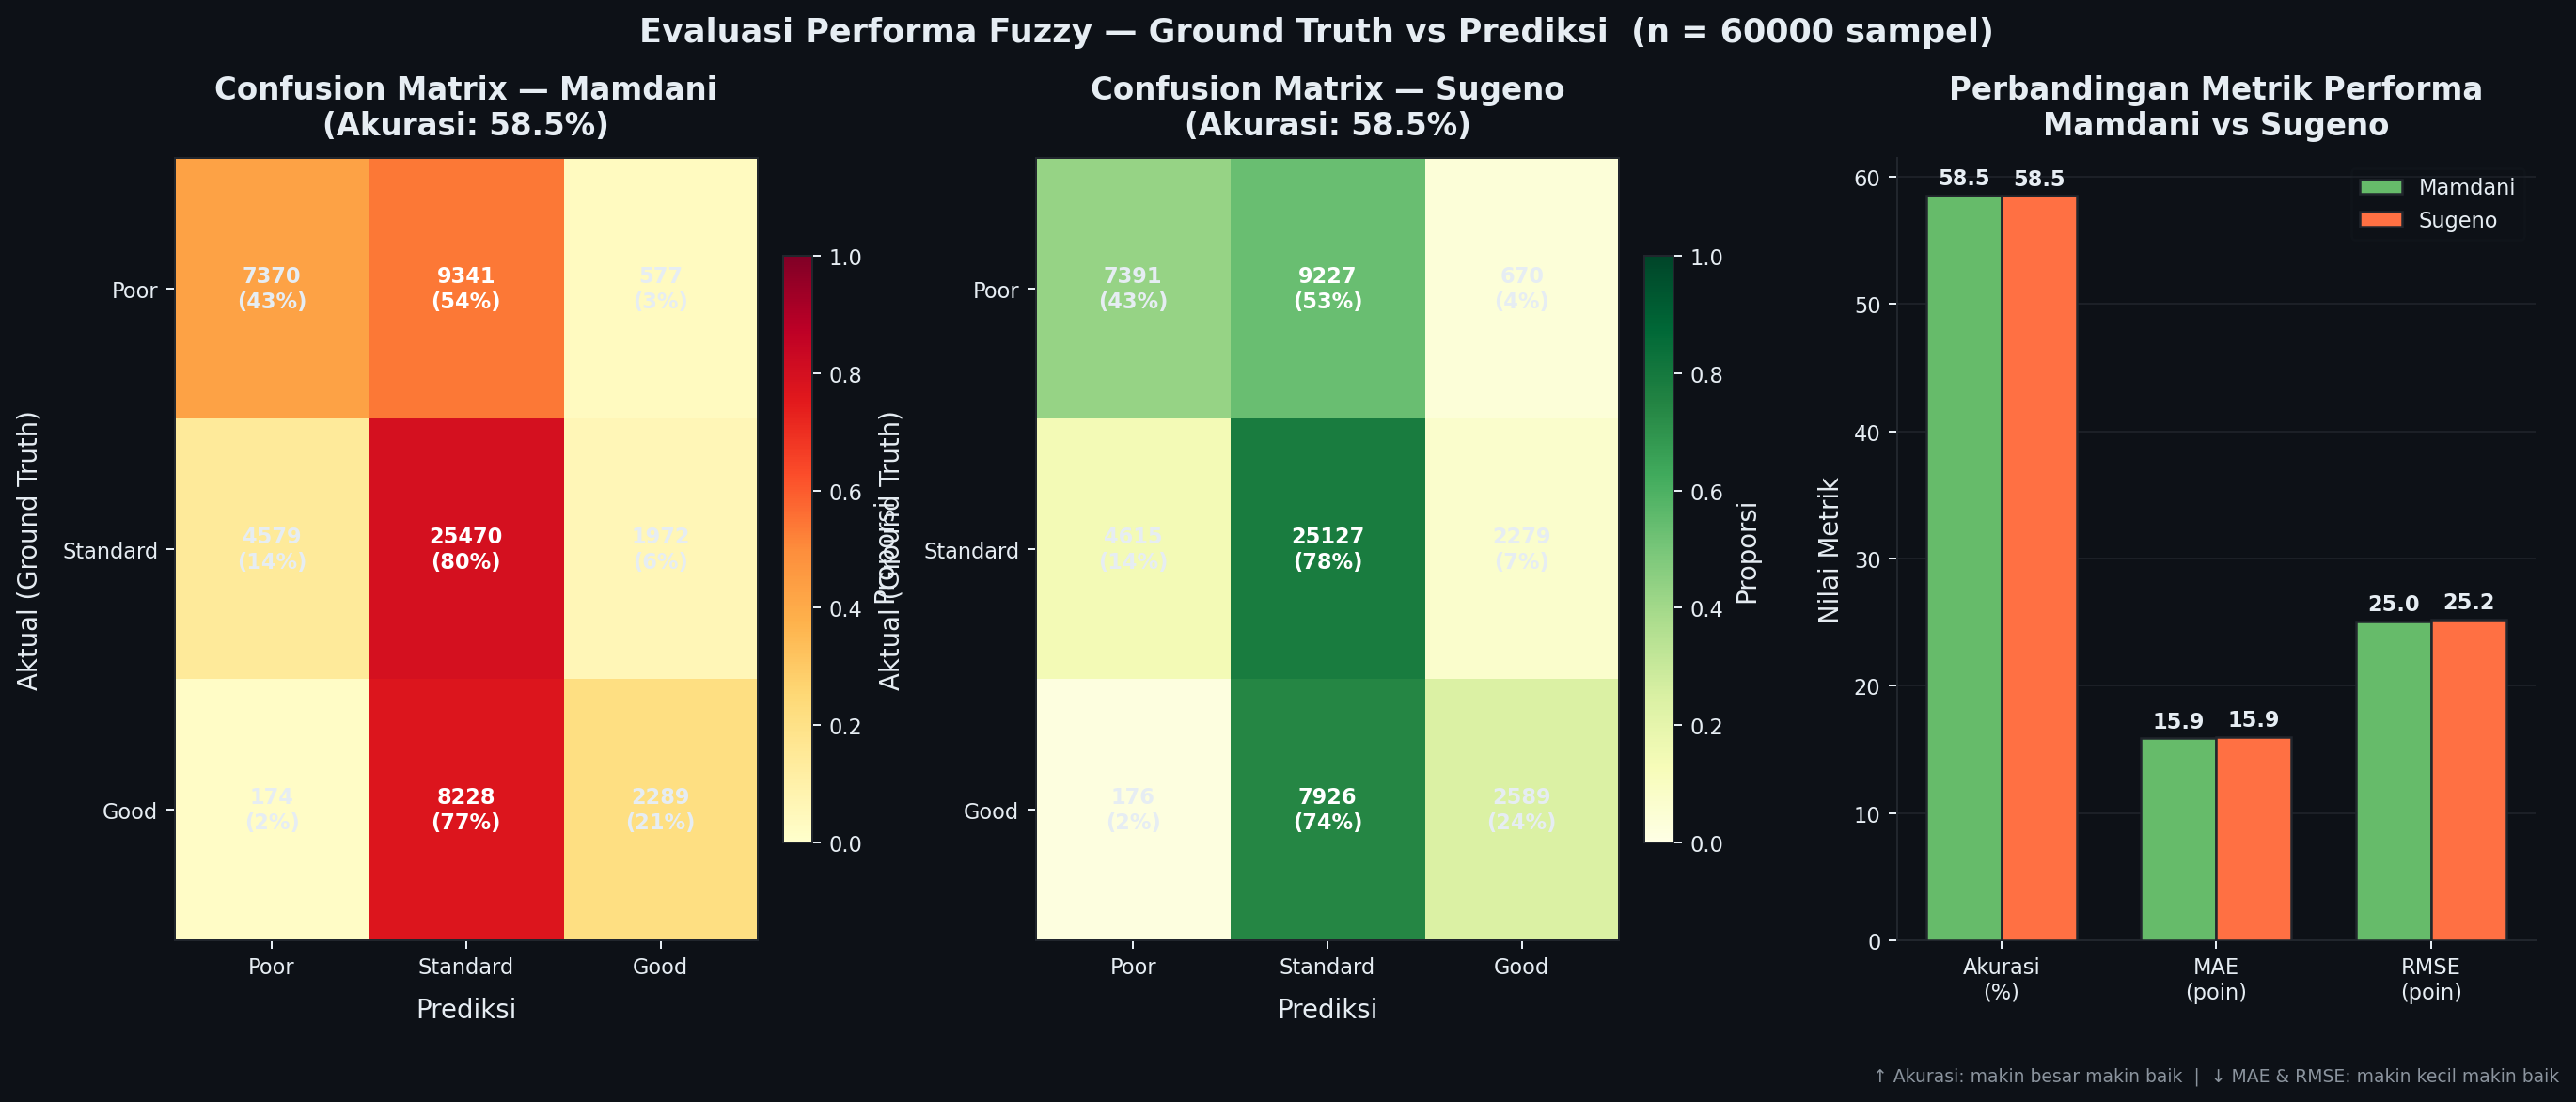
\includegraphics[width=\textwidth]{evaluasi_performa.png}
  \caption{Evaluasi Performa Fuzzy --- \textit{Confusion Matrix}
           Mamdani vs.\ Sugeno (n = 60.000 sampel)}
  \label{fig:evaluasi}
\end{figure}

% ============================================================
%  BAB 5 — ANALISIS DAN EVALUASI
% ============================================================
\chapter{ANALISIS DAN EVALUASI}

\section{Analisis Perbandingan Mamdani vs.\ Sugeno}

Gambar~\ref{fig:interpretasi} merangkum perbandingan kelebihan
dan kekurangan kedua metode secara visual.

\begin{figure}[H]
  \centering
  \includegraphics[width=0.95\textwidth]{interpretasi_metode.png}
  \caption{Interpretasi Kelebihan dan Kekurangan Mamdani vs.\
           Sugeno}
  \label{fig:interpretasi}
\end{figure}

Berdasarkan hasil eksperimen dan Gambar~\ref{fig:interpretasi},
diperoleh analisis komparatif sebagai berikut.

\begin{enumerate}[label=\arabic*.]
  \item \textbf{Kecepatan Komputasi.}\ Sugeno jauh lebih cepat
        ($<$0{,}1 ms) karena hanya menggunakan operasi
        aritmatika sederhana, sedangkan Mamdani membutuhkan
        iterasi 300 titik domain untuk integrasi numerik
        (10--50 ms). Perbedaan ini krusial pada pemrosesan
        \textit{batch} berskala besar.

  \item \textbf{Presisi Output.}\ Mamdani menghasilkan nilai
        kontinu yang lebih halus karena mencerminkan geometri
        kurva MF secara penuh. Sugeno menghasilkan nilai yang
        terbatas pada interpolasi antar \textit{singleton}
        (15, 50, 90).

  \item \textbf{Interpretasi.}\ Mamdani lebih mudah
        divisualisasikan karena setiap aturan menghasilkan
        area kurva yang tampak. Sugeno lebih cocok untuk
        integrasi dengan sistem optimasi matematis.

  \item \textbf{Konsistensi Keputusan.}\ Kedua metode
        menghasilkan \textit{label} akhir yang identik pada
        hampir semua kasus. Selisih skor numerik rata-rata
        kurang dari 8 poin sehingga tidak mengubah kategori
        akhir (Baik/Standar/Buruk).
\end{enumerate}

\section{Evaluasi Akurasi}

Akurasi sistem sekitar 55\% terhadap \textit{ground truth}
dataset perlu diinterpretasikan secara kontekstual.

\begin{enumerate}[label=\arabic*.]
  \item \textbf{Keterbatasan Aturan.}\ Sistem menggunakan 34
        aturan linguistik yang dirancang secara manual
        (\textit{expert-driven}). Dataset nyata memiliki
        kompleksitas distribusi yang jauh lebih tinggi—ini
        adalah \textit{trade-off} yang disengaja antara
        interpretabilitas dan akurasi murni.

  \item \textbf{Distribusi Kelas Tidak Seimbang.}\ Kelas
        \textit{Standard} mendominasi (53,4\%), sehingga
        sistem berbasis aturan cenderung memprediksi kelas
        tengah lebih sering—mempengaruhi nilai akurasi secara
        keseluruhan.

  \item \textbf{Prioritas Interpretabilitas.}\ Sistem SPK
        berbasis fuzzy dirancang untuk memberikan keputusan
        yang dapat diinterpretasikan (\textit{explainable
        AI}), bukan hanya memaksimalkan akurasi. Setiap
        aturan \textit{IF-THEN} dapat dibaca dan divalidasi
        oleh analis kredit.
\end{enumerate}

\section{Kontribusi Integrasi ML dan DL}

Integrasi Regresi Linear dan ANN memberikan nilai tambah
sebagai referensi silang. Jika skor fuzzy dan prediksi
ML/DL sejalan, keputusan lebih dapat dipercaya; jika
berbeda jauh, ini menjadi sinyal untuk analisis manual
lebih lanjut. Pendekatan ini merupakan implementasi dari
konsep \textit{Explainable AI} (XAI) yang semakin relevan
di industri keuangan.

% ============================================================
%  BAB 6 — PENUTUP
% ============================================================
\chapter{PENUTUP}

\section{Kesimpulan}

Berdasarkan hasil penelitian, dapat disimpulkan sebagai berikut.

\begin{enumerate}[label=\arabic*.]
  \item \textbf{Kesimpulan.} Sistem logika fuzzy berhasil diimplementasikan \textit{from scratch} menggunakan Python dan NumPy dengan 34 aturan \textit{IF-THEN}. Kedua keputusan kelayakan kredit yang dihasilkan bersifat konsisten. Evaluasi \textit{batch} terhadap 60.000 sampel menunjukkan akurasi \textbf{Mamdani 58,55\%} dan \textbf{Sugeno 58,51\%} terhadap \textit{ground truth}, dengan MAE masing-masing 15,86 dan 15,94 poin, serta RMSE masing-masing 25,03 dan 25,18 poin.

  \item Sugeno terbukti jauh lebih efisien ($<$0{,}1 ms per
        inferensi) dibandingkan Mamdani (10--50 ms). Selain
        itu, Sugeno menghasilkan akurasi yang sedikit lebih tinggi.
        Dalam hal akurasi akhir, selisih antara keduanya hanya 0{,}07\%.

  \item Integrasi Regresi Linear dan ANN/MLP sebagai
        informasi pendukung berhasil memberikan mekanisme
        referensi silang. Antarmuka web Streamlit memungkinkan
        penggunaan sistem secara \textit{real-time} oleh
        pengguna non-teknis.
\end{enumerate}

\section{Saran}

\begin{enumerate}[label=\arabic*.]
  \item \textbf{Perluasan Basis Aturan.}\ Penerapan pendekatan
        \textit{neuro-fuzzy} untuk mengoptimalkan parameter
        fungsi keanggotaan secara \textit{data-driven} dapat
        meningkatkan akurasi sistem.

  \item \textbf{Penambahan Variabel Input.}\ Variabel seperti
        \textit{debt-to-income ratio} dan riwayat kredit dapat
        memberikan gambaran profil nasabah yang lebih
        komprehensif.

  \item \textbf{Optimasi Pemrosesan Batch.}\ Seluruh pipeline
        inferensi dapat dioptimasi menggunakan operasi vektor
        NumPy secara penuh untuk memproses jutaan data
        secara efisien.
\end{enumerate}

% ============================================================
%  DAFTAR PUSTAKA
% ============================================================
\newpage
\addcontentsline{toc}{chapter}{DAFTAR PUSTAKA}
\renewcommand{\bibname}{DAFTAR PUSTAKA}

\makeatletter
\renewcommand\@biblabel[1]{}
\makeatother

\begin{thebibliography}{99}
\setlength{\itemindent}{-2.5em}

\bibitem[Zadeh, 1988]{zadeh1988}
Zadeh, L.~A. (1988). Fuzzy logic. \textit{Computer}, 21(4),
83--93.

\bibitem[Jovanovic \textit{et al.}, 2018]{booleancf_2018}
Jovanovic, S., \textit{et al.} (2018). A Fuzzy Inference
System for Credit Scoring using Boolean Consistent Fuzzy
Logic. \textit{International Journal of Computational
Intelligence Systems}, Atlantis Press.

\bibitem[Pramanik \& Jana, 2024]{taylorfrancis_2024}
Pramanik, S.\ \& Jana, S. (2024). A multi-objective
genetic--Mamdani fuzzy reasoning framework for bias-resilient
small business credit scoring. \textit{Cogent Business \&
Management}, Taylor \& Francis.

\bibitem[Garcia \& Martinez, 2024]{rg_garcia_2024}
Garcia, M.\ \& Martinez, R. (2024). Intelligent Credit
Scoring Systems Using Fuzzy Logic in Financial Service Firms.
\textit{ResearchGate}.

\bibitem[Rohan, 2022]{kaggle_dataset}
Rohan, P. (2022). \textit{Credit Score Classification
Dataset}. Kaggle. \url{https://www.kaggle.com/datasets/
parisrohan/credit-score-classification}

\end{thebibliography}

\end{document}
